% Created by tikzDevice version 0.10.1 on 2016-08-26 10:22:23
% !TEX encoding = UTF-8 Unicode
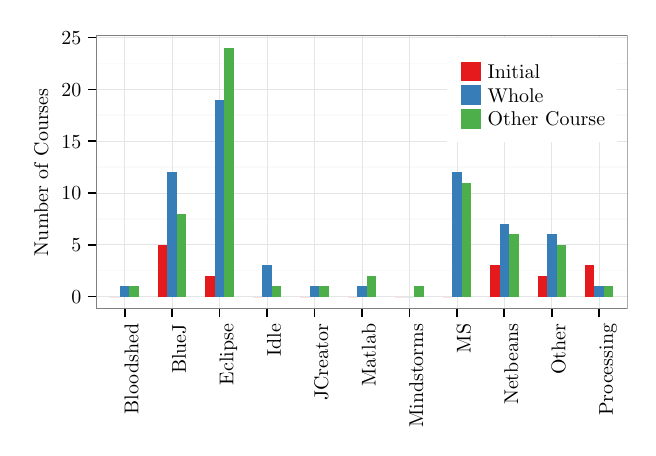
\begin{tikzpicture}[x=1pt,y=1pt]
\definecolor{fillColor}{RGB}{255,255,255}
\path[use as bounding box,fill=fillColor,fill opacity=0.00] (0,0) rectangle (216.81,144.54);
\begin{scope}
\path[clip] (  0.00,  0.00) rectangle (216.81,144.54);
\definecolor{drawColor}{RGB}{255,255,255}
\definecolor{fillColor}{RGB}{255,255,255}

\path[draw=drawColor,line width= 0.6pt,line join=round,line cap=round,fill=fillColor] (  0.00,  0.00) rectangle (216.81,144.54);
\end{scope}
\begin{scope}
\path[clip] ( 24.76, 42.89) rectangle (216.81,141.69);
\definecolor{fillColor}{RGB}{255,255,255}

\path[fill=fillColor] ( 24.76, 42.89) rectangle (216.81,141.69);
\definecolor{drawColor}{gray}{0.98}

\path[draw=drawColor,line width= 0.6pt,line join=round] ( 24.76, 56.74) --
	(216.81, 56.74);

\path[draw=drawColor,line width= 0.6pt,line join=round] ( 24.76, 75.45) --
	(216.81, 75.45);

\path[draw=drawColor,line width= 0.6pt,line join=round] ( 24.76, 94.16) --
	(216.81, 94.16);

\path[draw=drawColor,line width= 0.6pt,line join=round] ( 24.76,112.88) --
	(216.81,112.88);

\path[draw=drawColor,line width= 0.6pt,line join=round] ( 24.76,131.59) --
	(216.81,131.59);
\definecolor{drawColor}{gray}{0.90}

\path[draw=drawColor,line width= 0.2pt,line join=round] ( 24.76, 47.38) --
	(216.81, 47.38);

\path[draw=drawColor,line width= 0.2pt,line join=round] ( 24.76, 66.09) --
	(216.81, 66.09);

\path[draw=drawColor,line width= 0.2pt,line join=round] ( 24.76, 84.81) --
	(216.81, 84.81);

\path[draw=drawColor,line width= 0.2pt,line join=round] ( 24.76,103.52) --
	(216.81,103.52);

\path[draw=drawColor,line width= 0.2pt,line join=round] ( 24.76,122.23) --
	(216.81,122.23);

\path[draw=drawColor,line width= 0.2pt,line join=round] ( 24.76,140.95) --
	(216.81,140.95);

\path[draw=drawColor,line width= 0.2pt,line join=round] ( 35.05, 42.89) --
	( 35.05,141.69);

\path[draw=drawColor,line width= 0.2pt,line join=round] ( 52.19, 42.89) --
	( 52.19,141.69);

\path[draw=drawColor,line width= 0.2pt,line join=round] ( 69.34, 42.89) --
	( 69.34,141.69);

\path[draw=drawColor,line width= 0.2pt,line join=round] ( 86.49, 42.89) --
	( 86.49,141.69);

\path[draw=drawColor,line width= 0.2pt,line join=round] (103.64, 42.89) --
	(103.64,141.69);

\path[draw=drawColor,line width= 0.2pt,line join=round] (120.78, 42.89) --
	(120.78,141.69);

\path[draw=drawColor,line width= 0.2pt,line join=round] (137.93, 42.89) --
	(137.93,141.69);

\path[draw=drawColor,line width= 0.2pt,line join=round] (155.08, 42.89) --
	(155.08,141.69);

\path[draw=drawColor,line width= 0.2pt,line join=round] (172.23, 42.89) --
	(172.23,141.69);

\path[draw=drawColor,line width= 0.2pt,line join=round] (189.37, 42.89) --
	(189.37,141.69);

\path[draw=drawColor,line width= 0.2pt,line join=round] (206.52, 42.89) --
	(206.52,141.69);
\definecolor{fillColor}{RGB}{228,26,28}

\path[fill=fillColor] ( 29.90, 47.38) rectangle ( 33.33, 47.38);
\definecolor{fillColor}{RGB}{55,126,184}

\path[fill=fillColor] ( 33.33, 47.38) rectangle ( 36.76, 51.12);
\definecolor{fillColor}{RGB}{77,175,74}

\path[fill=fillColor] ( 36.76, 47.38) rectangle ( 40.19, 51.12);
\definecolor{fillColor}{RGB}{228,26,28}

\path[fill=fillColor] ( 47.05, 47.38) rectangle ( 50.48, 66.09);
\definecolor{fillColor}{RGB}{55,126,184}

\path[fill=fillColor] ( 50.48, 47.38) rectangle ( 53.91, 92.29);
\definecolor{fillColor}{RGB}{77,175,74}

\path[fill=fillColor] ( 53.91, 47.38) rectangle ( 57.34, 77.32);
\definecolor{fillColor}{RGB}{228,26,28}

\path[fill=fillColor] ( 64.20, 47.38) rectangle ( 67.63, 54.87);
\definecolor{fillColor}{RGB}{55,126,184}

\path[fill=fillColor] ( 67.63, 47.38) rectangle ( 71.06,118.49);
\definecolor{fillColor}{RGB}{77,175,74}

\path[fill=fillColor] ( 71.06, 47.38) rectangle ( 74.49,137.20);
\definecolor{fillColor}{RGB}{228,26,28}

\path[fill=fillColor] ( 81.34, 47.38) rectangle ( 84.77, 47.38);
\definecolor{fillColor}{RGB}{55,126,184}

\path[fill=fillColor] ( 84.77, 47.38) rectangle ( 88.20, 58.61);
\definecolor{fillColor}{RGB}{77,175,74}

\path[fill=fillColor] ( 88.20, 47.38) rectangle ( 91.63, 51.12);
\definecolor{fillColor}{RGB}{228,26,28}

\path[fill=fillColor] ( 98.49, 47.38) rectangle (101.92, 47.38);
\definecolor{fillColor}{RGB}{55,126,184}

\path[fill=fillColor] (101.92, 47.38) rectangle (105.35, 51.12);
\definecolor{fillColor}{RGB}{77,175,74}

\path[fill=fillColor] (105.35, 47.38) rectangle (108.78, 51.12);
\definecolor{fillColor}{RGB}{228,26,28}

\path[fill=fillColor] (115.64, 47.38) rectangle (119.07, 47.38);
\definecolor{fillColor}{RGB}{55,126,184}

\path[fill=fillColor] (119.07, 47.38) rectangle (122.50, 51.12);
\definecolor{fillColor}{RGB}{77,175,74}

\path[fill=fillColor] (122.50, 47.38) rectangle (125.93, 54.87);
\definecolor{fillColor}{RGB}{228,26,28}

\path[fill=fillColor] (132.79, 47.38) rectangle (136.22, 47.38);
\definecolor{fillColor}{RGB}{55,126,184}

\path[fill=fillColor] (136.22, 47.38) rectangle (139.65, 47.38);
\definecolor{fillColor}{RGB}{77,175,74}

\path[fill=fillColor] (139.65, 47.38) rectangle (143.08, 51.12);
\definecolor{fillColor}{RGB}{228,26,28}

\path[fill=fillColor] (149.93, 47.38) rectangle (153.36, 47.38);
\definecolor{fillColor}{RGB}{55,126,184}

\path[fill=fillColor] (153.36, 47.38) rectangle (156.79, 92.29);
\definecolor{fillColor}{RGB}{77,175,74}

\path[fill=fillColor] (156.79, 47.38) rectangle (160.22, 88.55);
\definecolor{fillColor}{RGB}{228,26,28}

\path[fill=fillColor] (167.08, 47.38) rectangle (170.51, 58.61);
\definecolor{fillColor}{RGB}{55,126,184}

\path[fill=fillColor] (170.51, 47.38) rectangle (173.94, 73.58);
\definecolor{fillColor}{RGB}{77,175,74}

\path[fill=fillColor] (173.94, 47.38) rectangle (177.37, 69.84);
\definecolor{fillColor}{RGB}{228,26,28}

\path[fill=fillColor] (184.23, 47.38) rectangle (187.66, 54.87);
\definecolor{fillColor}{RGB}{55,126,184}

\path[fill=fillColor] (187.66, 47.38) rectangle (191.09, 69.84);
\definecolor{fillColor}{RGB}{77,175,74}

\path[fill=fillColor] (191.09, 47.38) rectangle (194.52, 66.09);
\definecolor{fillColor}{RGB}{228,26,28}

\path[fill=fillColor] (201.38, 47.38) rectangle (204.81, 58.61);
\definecolor{fillColor}{RGB}{55,126,184}

\path[fill=fillColor] (204.81, 47.38) rectangle (208.24, 51.12);
\definecolor{fillColor}{RGB}{77,175,74}

\path[fill=fillColor] (208.24, 47.38) rectangle (211.67, 51.12);
\definecolor{drawColor}{gray}{0.50}

\path[draw=drawColor,line width= 0.6pt,line join=round,line cap=round] ( 24.76, 42.89) rectangle (216.81,141.69);
\end{scope}
\begin{scope}
\path[clip] (  0.00,  0.00) rectangle (216.81,144.54);
\definecolor{drawColor}{RGB}{0,0,0}

\node[text=drawColor,anchor=base east,inner sep=0pt, outer sep=0pt, scale=  0.72] at ( 19.36, 44.90) {0};

\node[text=drawColor,anchor=base east,inner sep=0pt, outer sep=0pt, scale=  0.72] at ( 19.36, 63.62) {5};

\node[text=drawColor,anchor=base east,inner sep=0pt, outer sep=0pt, scale=  0.72] at ( 19.36, 82.33) {10};

\node[text=drawColor,anchor=base east,inner sep=0pt, outer sep=0pt, scale=  0.72] at ( 19.36,101.04) {15};

\node[text=drawColor,anchor=base east,inner sep=0pt, outer sep=0pt, scale=  0.72] at ( 19.36,119.75) {20};

\node[text=drawColor,anchor=base east,inner sep=0pt, outer sep=0pt, scale=  0.72] at ( 19.36,138.47) {25};
\end{scope}
\begin{scope}
\path[clip] (  0.00,  0.00) rectangle (216.81,144.54);
\definecolor{drawColor}{RGB}{0,0,0}

\path[draw=drawColor,line width= 0.6pt,line join=round] ( 21.76, 47.38) --
	( 24.76, 47.38);

\path[draw=drawColor,line width= 0.6pt,line join=round] ( 21.76, 66.09) --
	( 24.76, 66.09);

\path[draw=drawColor,line width= 0.6pt,line join=round] ( 21.76, 84.81) --
	( 24.76, 84.81);

\path[draw=drawColor,line width= 0.6pt,line join=round] ( 21.76,103.52) --
	( 24.76,103.52);

\path[draw=drawColor,line width= 0.6pt,line join=round] ( 21.76,122.23) --
	( 24.76,122.23);

\path[draw=drawColor,line width= 0.6pt,line join=round] ( 21.76,140.95) --
	( 24.76,140.95);
\end{scope}
\begin{scope}
\path[clip] (  0.00,  0.00) rectangle (216.81,144.54);
\definecolor{drawColor}{RGB}{0,0,0}

\path[draw=drawColor,line width= 0.6pt,line join=round] ( 35.05, 39.89) --
	( 35.05, 42.89);

\path[draw=drawColor,line width= 0.6pt,line join=round] ( 52.19, 39.89) --
	( 52.19, 42.89);

\path[draw=drawColor,line width= 0.6pt,line join=round] ( 69.34, 39.89) --
	( 69.34, 42.89);

\path[draw=drawColor,line width= 0.6pt,line join=round] ( 86.49, 39.89) --
	( 86.49, 42.89);

\path[draw=drawColor,line width= 0.6pt,line join=round] (103.64, 39.89) --
	(103.64, 42.89);

\path[draw=drawColor,line width= 0.6pt,line join=round] (120.78, 39.89) --
	(120.78, 42.89);

\path[draw=drawColor,line width= 0.6pt,line join=round] (137.93, 39.89) --
	(137.93, 42.89);

\path[draw=drawColor,line width= 0.6pt,line join=round] (155.08, 39.89) --
	(155.08, 42.89);

\path[draw=drawColor,line width= 0.6pt,line join=round] (172.23, 39.89) --
	(172.23, 42.89);

\path[draw=drawColor,line width= 0.6pt,line join=round] (189.37, 39.89) --
	(189.37, 42.89);

\path[draw=drawColor,line width= 0.6pt,line join=round] (206.52, 39.89) --
	(206.52, 42.89);
\end{scope}
\begin{scope}
\path[clip] (  0.00,  0.00) rectangle (216.81,144.54);
\definecolor{drawColor}{RGB}{0,0,0}

\node[text=drawColor,rotate= 90.00,anchor=base east,inner sep=0pt, outer sep=0pt, scale=  0.72] at ( 40.00, 37.49) {Bloodshed};

\node[text=drawColor,rotate= 90.00,anchor=base east,inner sep=0pt, outer sep=0pt, scale=  0.72] at ( 57.15, 37.49) {BlueJ};

\node[text=drawColor,rotate= 90.00,anchor=base east,inner sep=0pt, outer sep=0pt, scale=  0.72] at ( 74.30, 37.49) {Eclipse};

\node[text=drawColor,rotate= 90.00,anchor=base east,inner sep=0pt, outer sep=0pt, scale=  0.72] at ( 91.45, 37.49) {Idle};

\node[text=drawColor,rotate= 90.00,anchor=base east,inner sep=0pt, outer sep=0pt, scale=  0.72] at (108.59, 37.49) {JCreator};

\node[text=drawColor,rotate= 90.00,anchor=base east,inner sep=0pt, outer sep=0pt, scale=  0.72] at (125.74, 37.49) {Matlab};

\node[text=drawColor,rotate= 90.00,anchor=base east,inner sep=0pt, outer sep=0pt, scale=  0.72] at (142.89, 37.49) {Mindstorms};

\node[text=drawColor,rotate= 90.00,anchor=base east,inner sep=0pt, outer sep=0pt, scale=  0.72] at (160.04, 37.49) {MS};

\node[text=drawColor,rotate= 90.00,anchor=base east,inner sep=0pt, outer sep=0pt, scale=  0.72] at (177.19, 37.49) {Netbeans};

\node[text=drawColor,rotate= 90.00,anchor=base east,inner sep=0pt, outer sep=0pt, scale=  0.72] at (194.33, 37.49) {Other};

\node[text=drawColor,rotate= 90.00,anchor=base east,inner sep=0pt, outer sep=0pt, scale=  0.72] at (211.48, 37.49) {Processing};
\end{scope}
\begin{scope}
\path[clip] (  0.00,  0.00) rectangle (216.81,144.54);
\definecolor{drawColor}{RGB}{0,0,0}

\node[text=drawColor,rotate= 90.00,anchor=base,inner sep=0pt, outer sep=0pt, scale=  0.72] at (  7.36, 92.29) {Number of Courses};
\end{scope}
\begin{scope}
\path[clip] (  0.00,  0.00) rectangle (216.81,144.54);
\definecolor{fillColor}{RGB}{255,255,255}

\path[fill=fillColor] (151.57,103.06) rectangle (212.91,140.81);
\end{scope}
\begin{scope}
\path[clip] (  0.00,  0.00) rectangle (216.81,144.54);
\definecolor{fillColor}{RGB}{228,26,28}

\path[fill=fillColor] (156.55,125.11) rectangle (163.66,132.22);
\end{scope}
\begin{scope}
\path[clip] (  0.00,  0.00) rectangle (216.81,144.54);
\definecolor{fillColor}{RGB}{55,126,184}

\path[fill=fillColor] (156.55,116.57) rectangle (163.66,123.68);
\end{scope}
\begin{scope}
\path[clip] (  0.00,  0.00) rectangle (216.81,144.54);
\definecolor{fillColor}{RGB}{77,175,74}

\path[fill=fillColor] (156.55,108.03) rectangle (163.66,115.15);
\end{scope}
\begin{scope}
\path[clip] (  0.00,  0.00) rectangle (216.81,144.54);
\definecolor{drawColor}{RGB}{0,0,0}

\node[text=drawColor,anchor=base west,inner sep=0pt, outer sep=0pt, scale=  0.72] at (166.18,126.18) {Initial};
\end{scope}
\begin{scope}
\path[clip] (  0.00,  0.00) rectangle (216.81,144.54);
\definecolor{drawColor}{RGB}{0,0,0}

\node[text=drawColor,anchor=base west,inner sep=0pt, outer sep=0pt, scale=  0.72] at (166.18,117.65) {Whole};
\end{scope}
\begin{scope}
\path[clip] (  0.00,  0.00) rectangle (216.81,144.54);
\definecolor{drawColor}{RGB}{0,0,0}

\node[text=drawColor,anchor=base west,inner sep=0pt, outer sep=0pt, scale=  0.72] at (166.18,109.11) {Other Course};
\end{scope}
\end{tikzpicture}
